 \chapter{Design}

\section{Overall System Design}

\subsection{Short description of the main parts of the system}

\begin {itemize}
	\item Main Parts
	\begin {itemize}
		\item Database View Interface
		\begin {itemize}
			\item Presented as a database window with 6 push buttons that open dialog boxes for different functions
			\item the 6 push buttons are labelled:
			\begin {itemize}
				\item Open
				\item Add
				\item Edit
				\item delete
				\item Search
				\item Print
			\end {itemize}
		\item Each table in the database is displayed in a different tab
		\item Main window displays database in a box above function buttons
		\item Has a menu bar at the top that provides shortcuts to the functions and an about section with a help section that contains   a user manual
	\item Open Interface
	\begin {itemize}
		\item Two push buttons - open file and close
		\item 1st button opens the file browser to chose a database to open
		\item 2nd button closes the dialog button
	\end {itemize}
	\item Add Interface
	\begin {itemize}
		\item Drop down menu to select table
		\item Fields with editable text boxes/line edits to enter attributes
		\item confirm button
	\end {itemize}
	\item Edit Interface
    \begin {itemize}
		\item Drop down menu to select table
		\item Fields with editable text boxes/line edits to enter attributes
		\item confirm button
	\end {itemize}
	\item Delete Interface
	\begin {itemize}
		\item Select table drop down menu
		\item Select item drop down menu
		\item Delete button
		\item Delete all itmes button
		\item require a password to b entered first in a dialog box
	\end {itemize}
	\item Search Interface
	\begin {itemize}
		\item Select table drop down menu
		\item Search term QLineEdit
		\item Search push button
	\end {itemize}	
	\end {itemize}
	\end {itemize}
\end {itemize}

\subsection{System flowcharts showing an overview of the complete system}

\begin{figure}[H]
    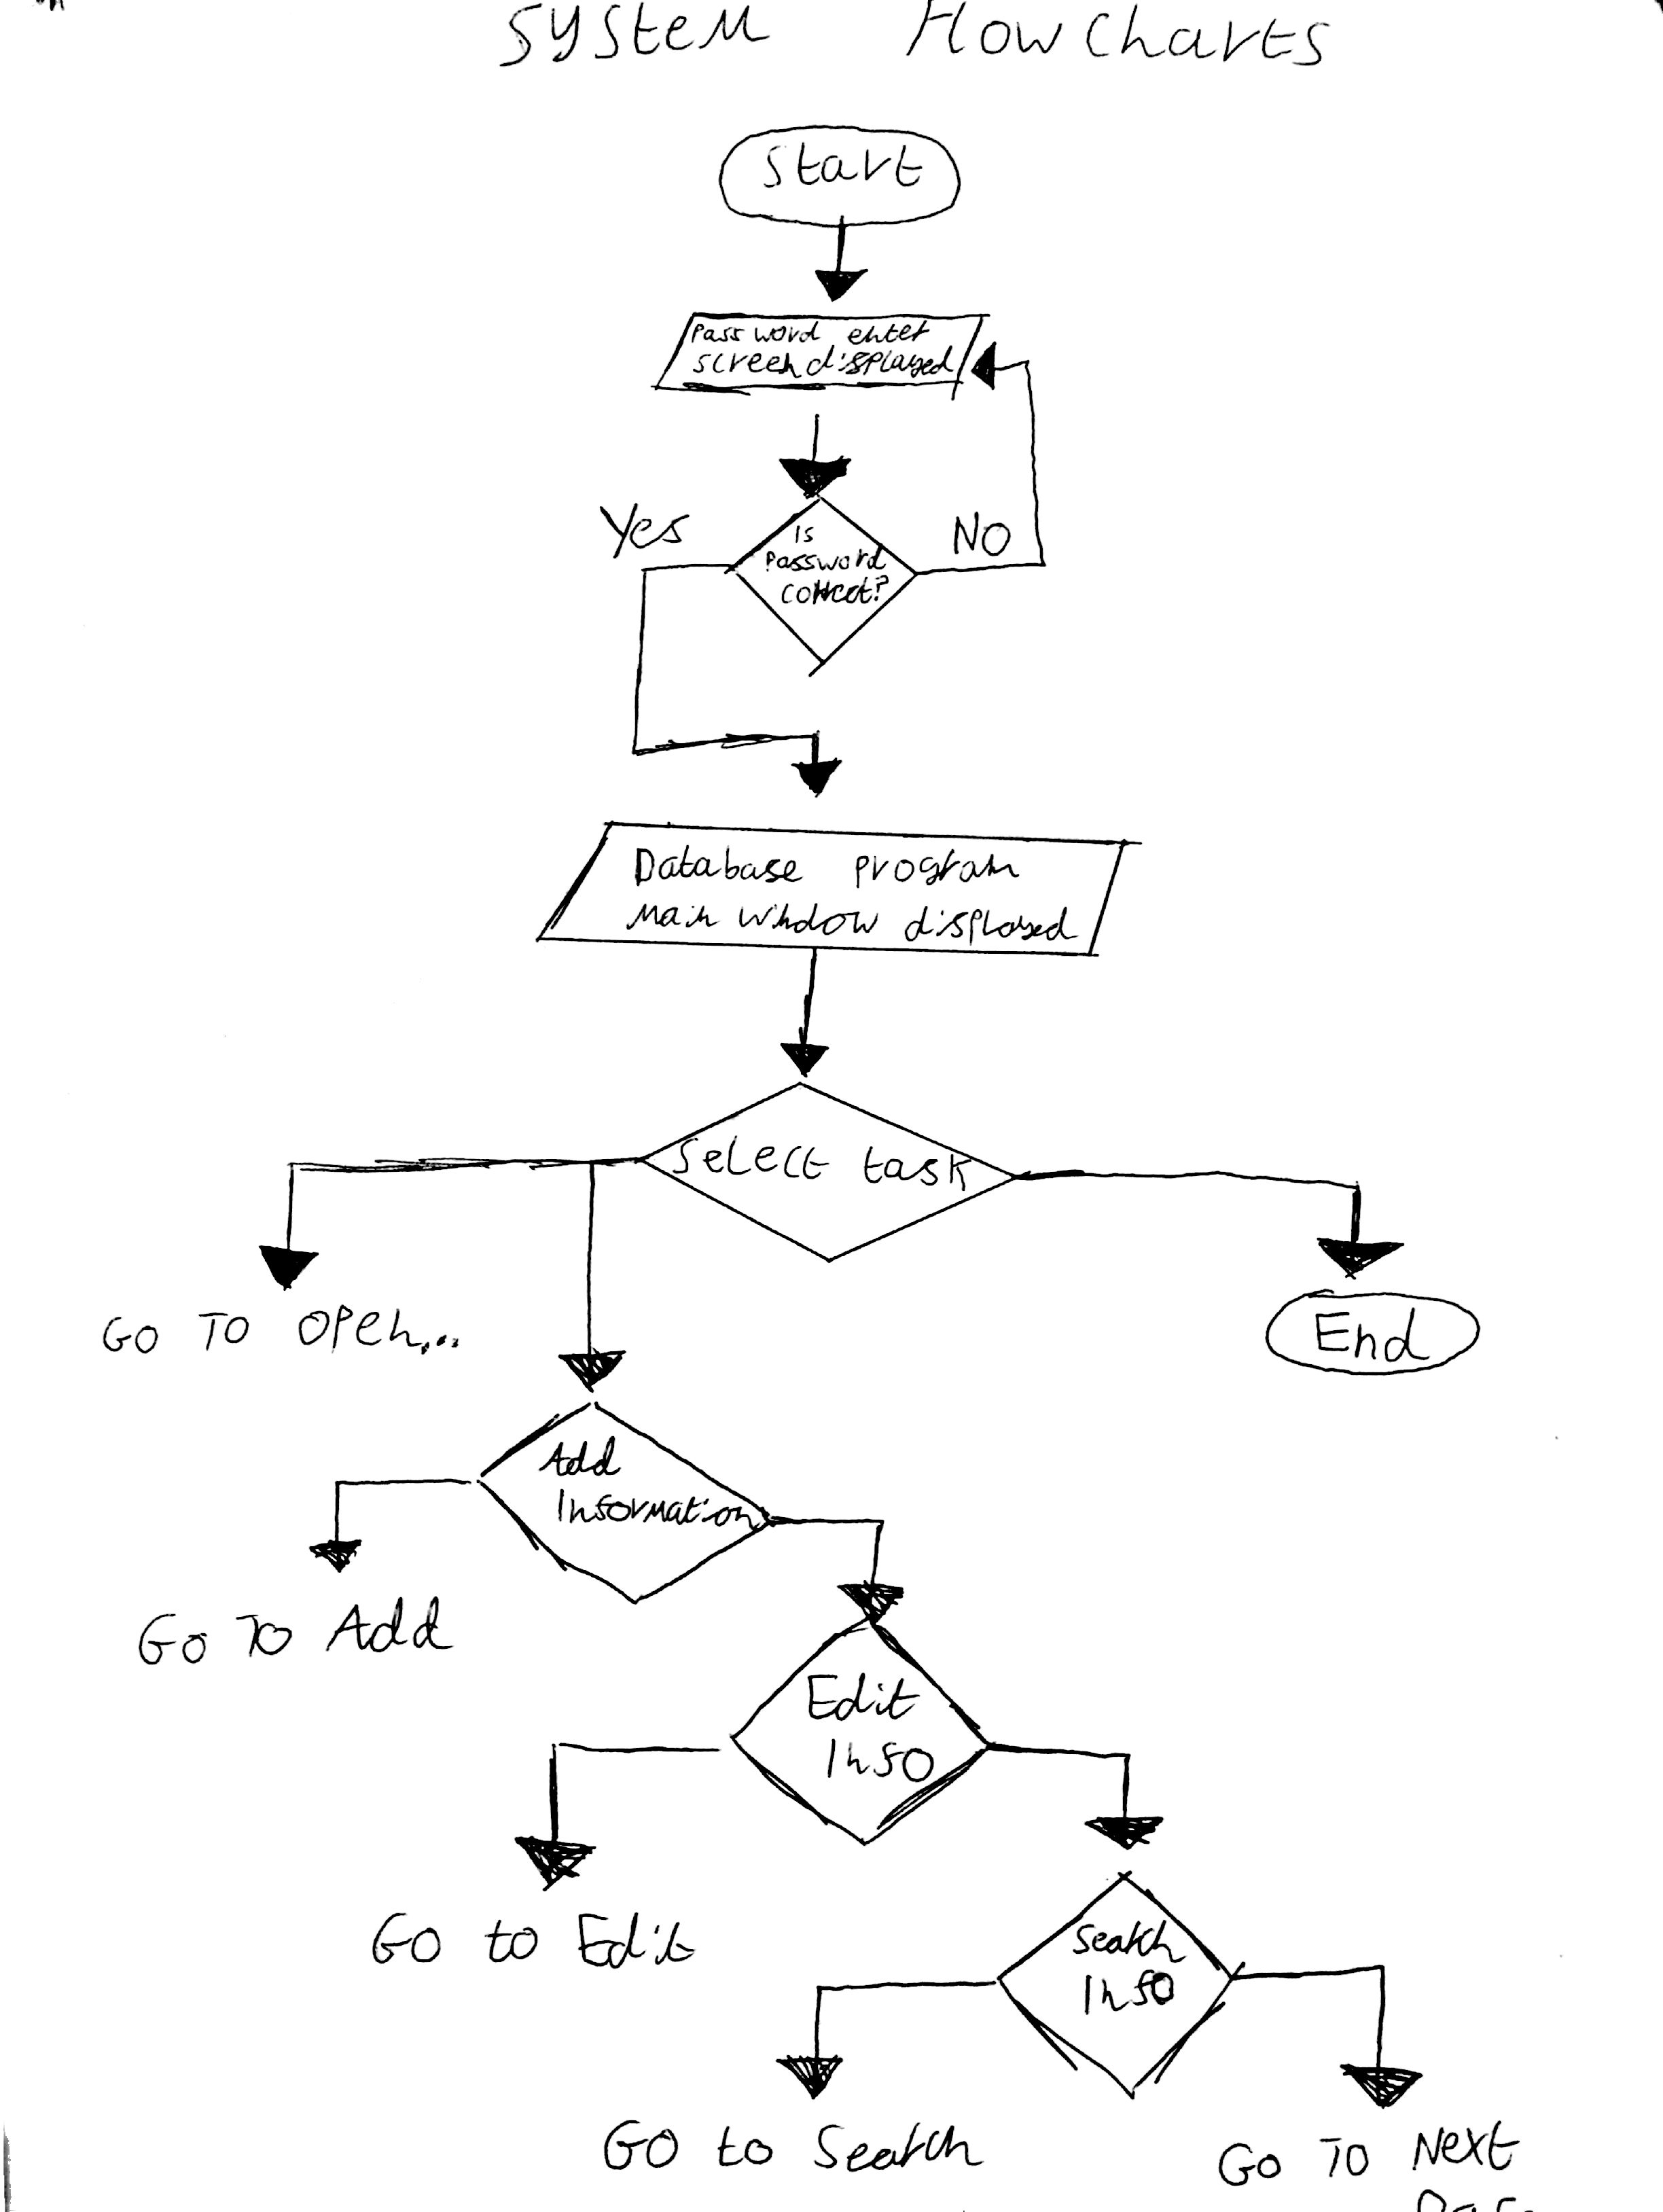
\includegraphics[width=\textwidth]{flowchart 5.jpg}
    \caption{Flowchart} \label{fig:Flowchart}
\end{figure}


\begin{figure}[H]
    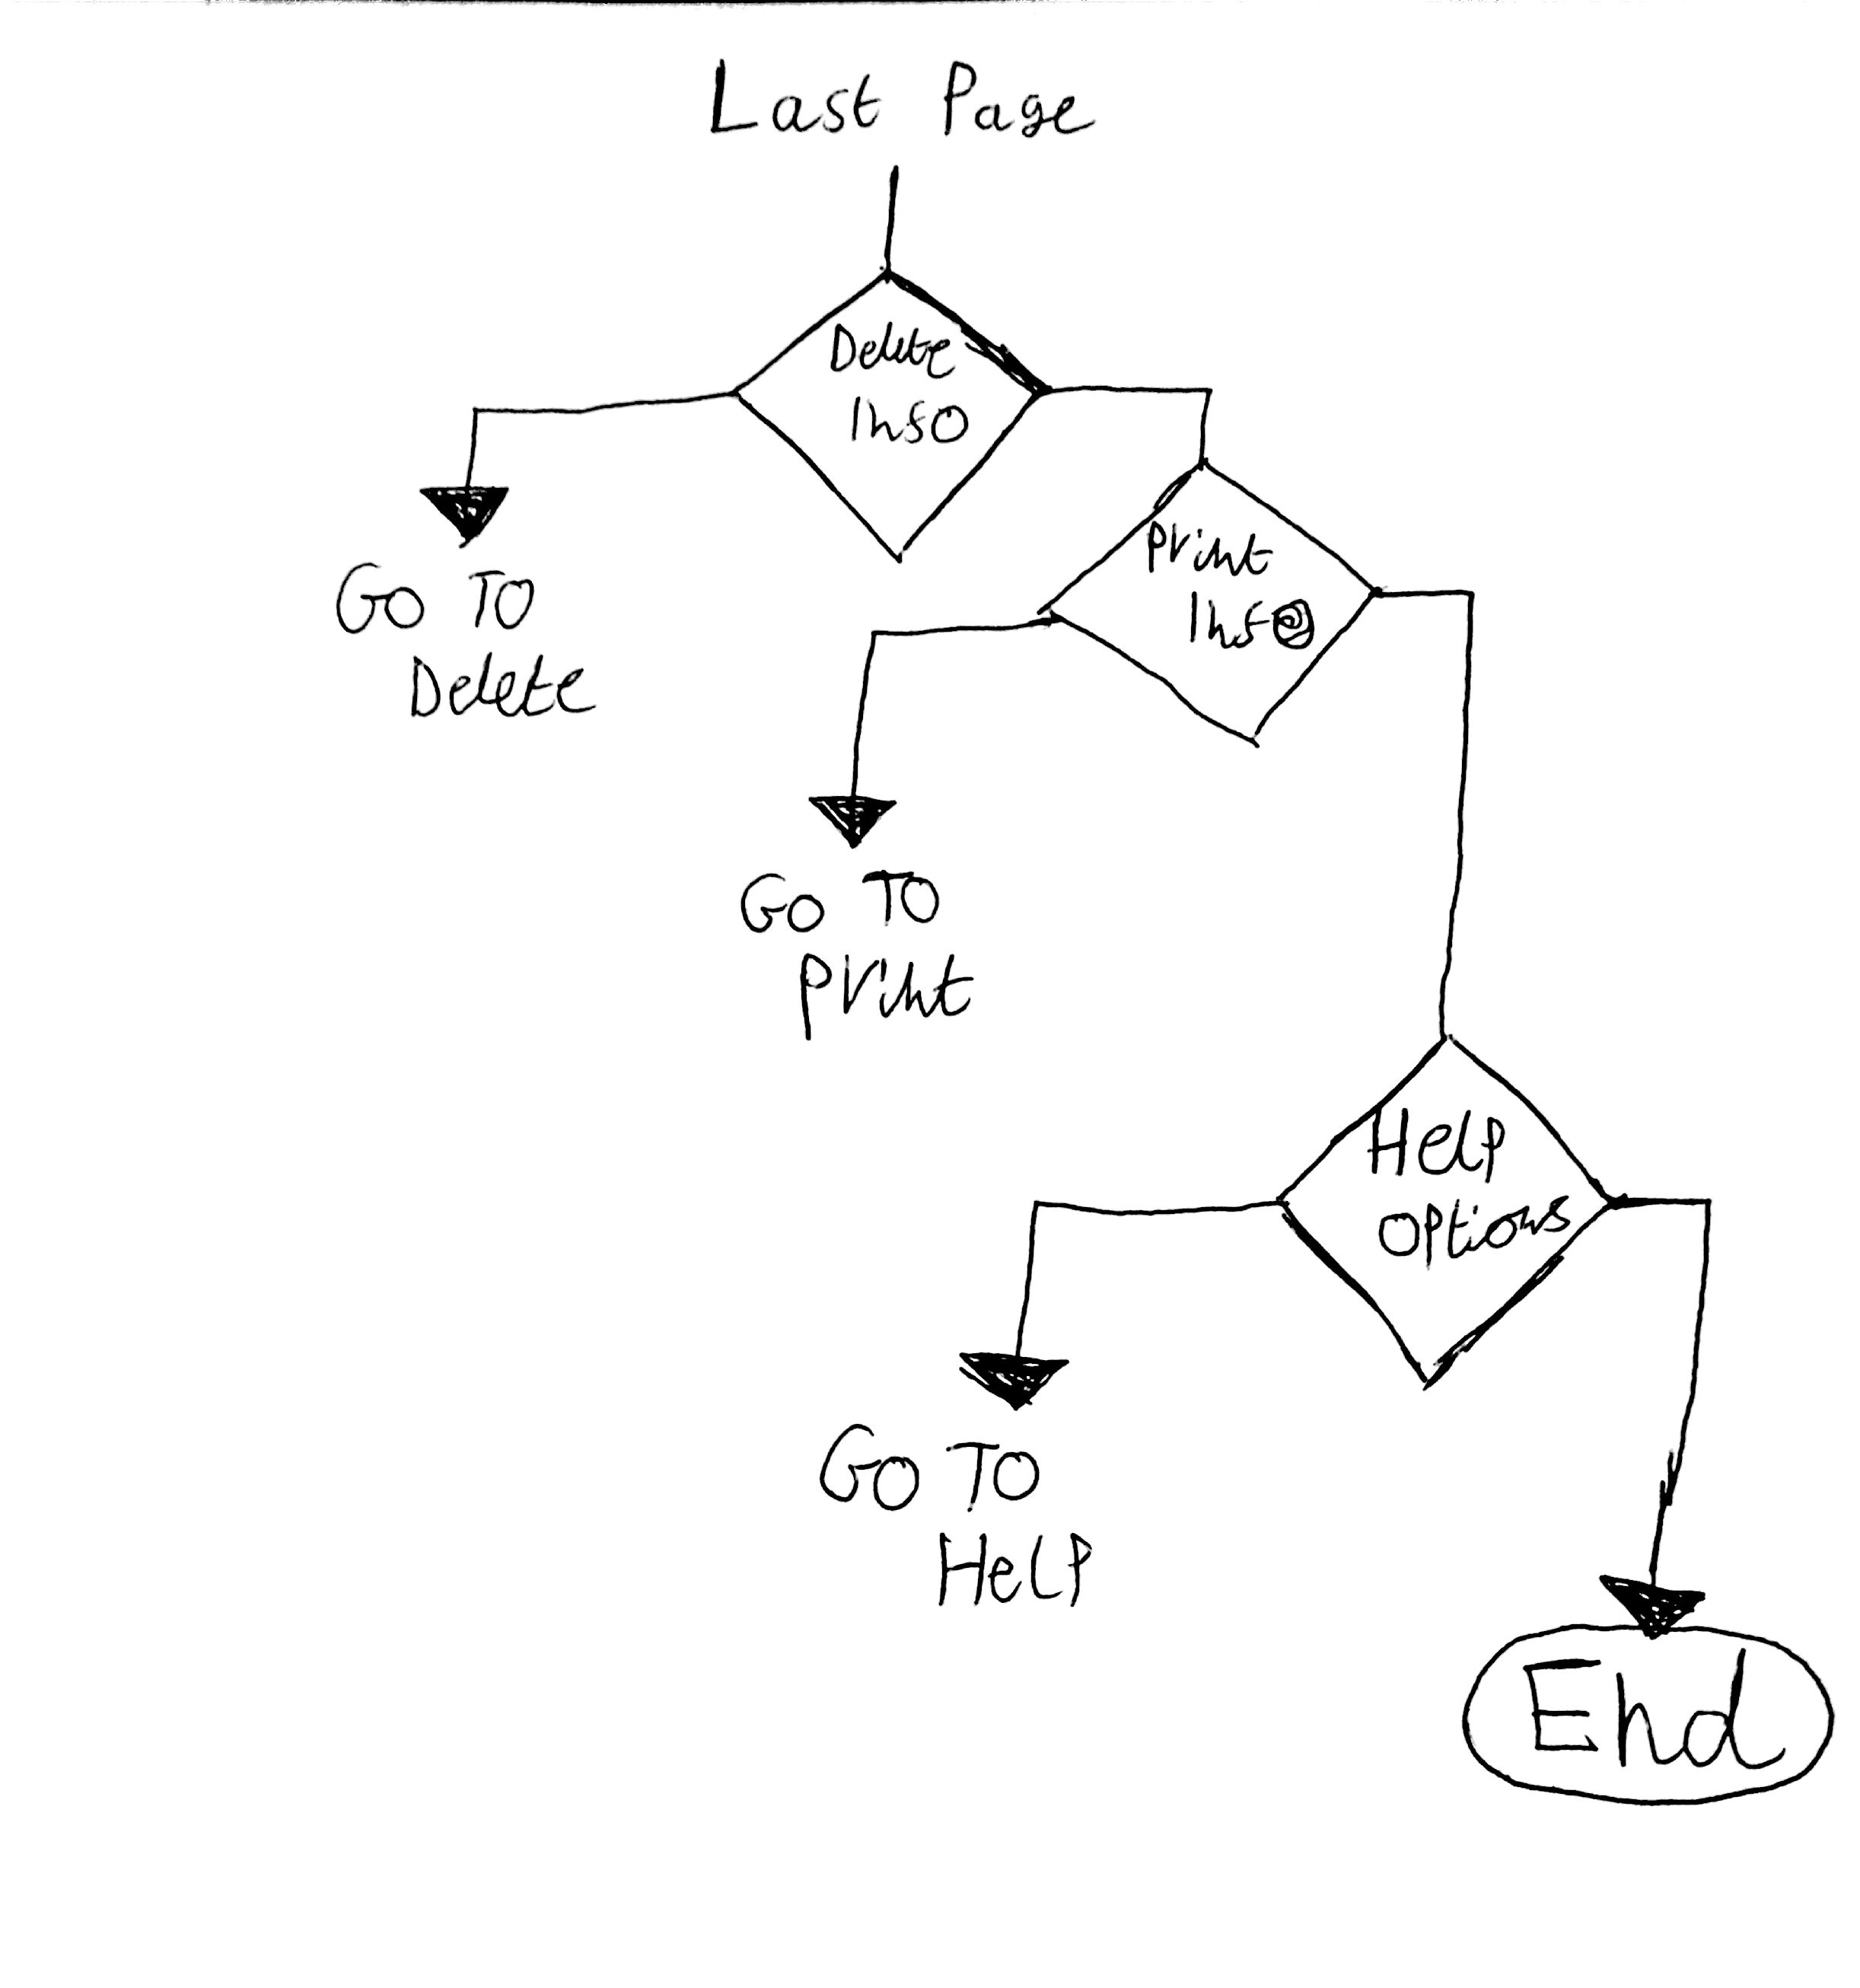
\includegraphics[width=\textwidth]{flowchart4.jpg}
    \caption{Flowchart} \label{fig:Flowchart}
\end{figure}

\begin{figure}[H]
    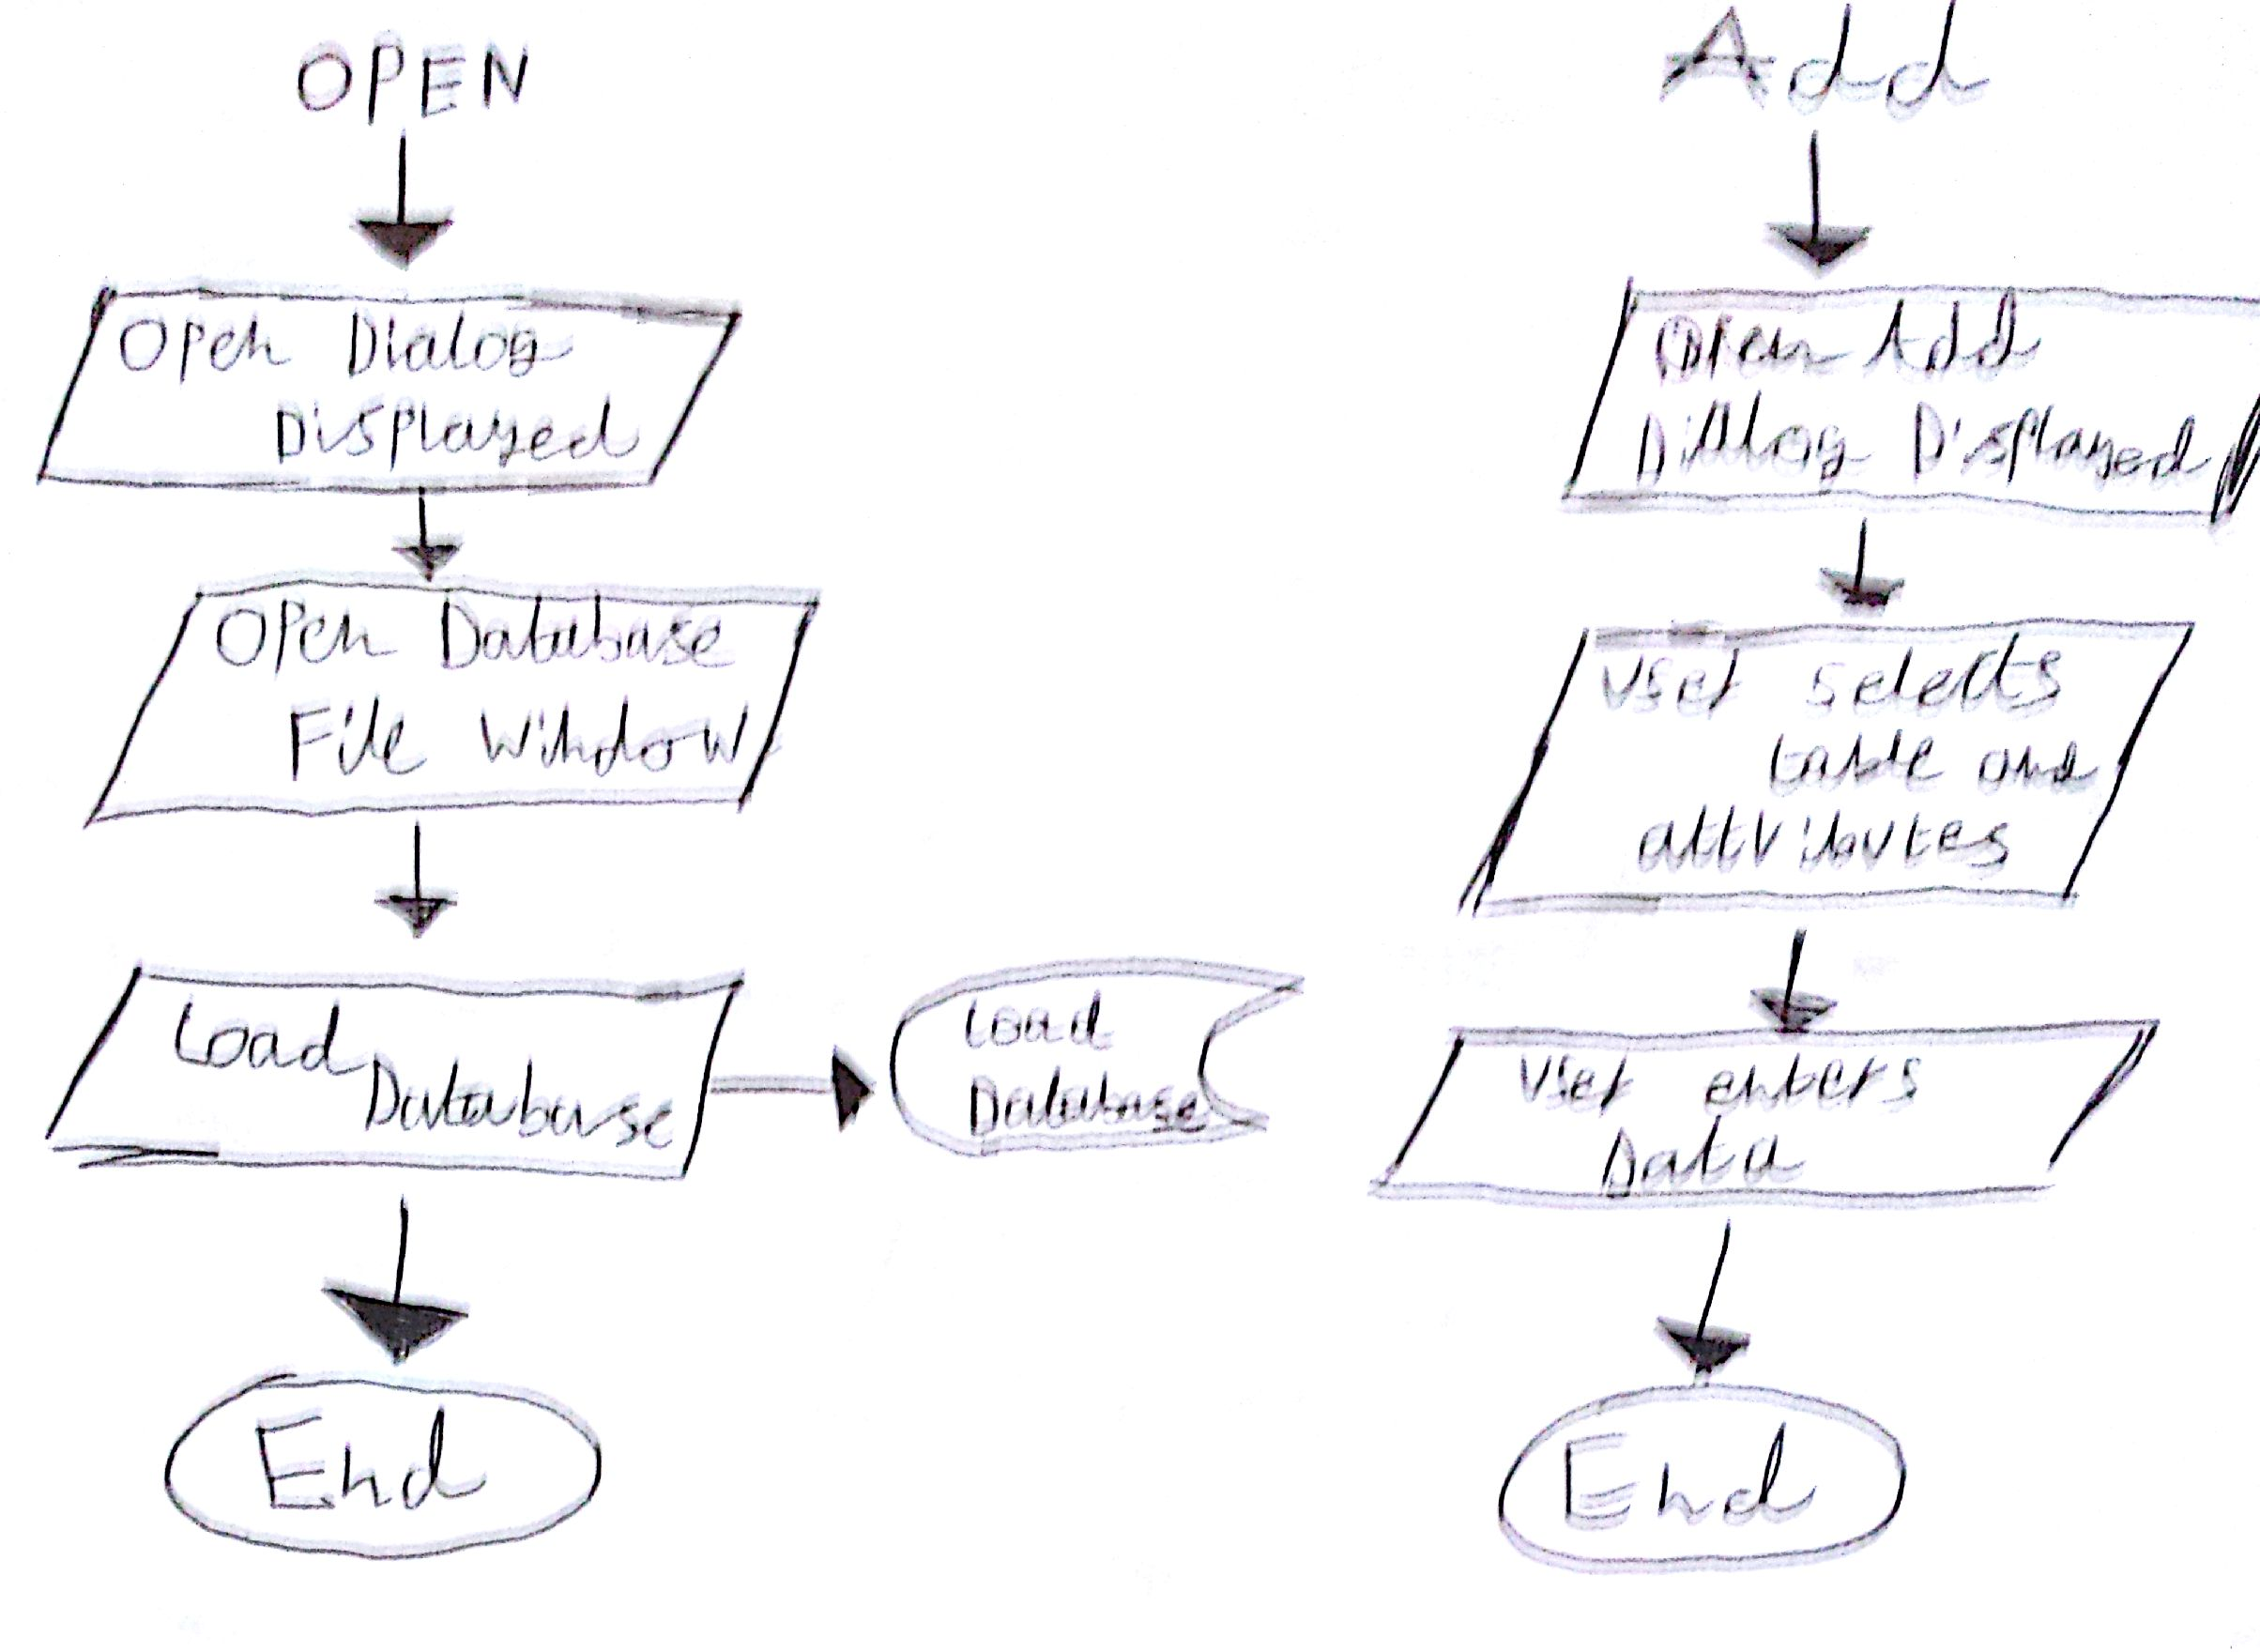
\includegraphics[width=\textwidth]{flowchart3.jpg}
    \caption{Flowchart} \label{fig:Flowchart}
\end{figure}

\begin{figure}[H]
    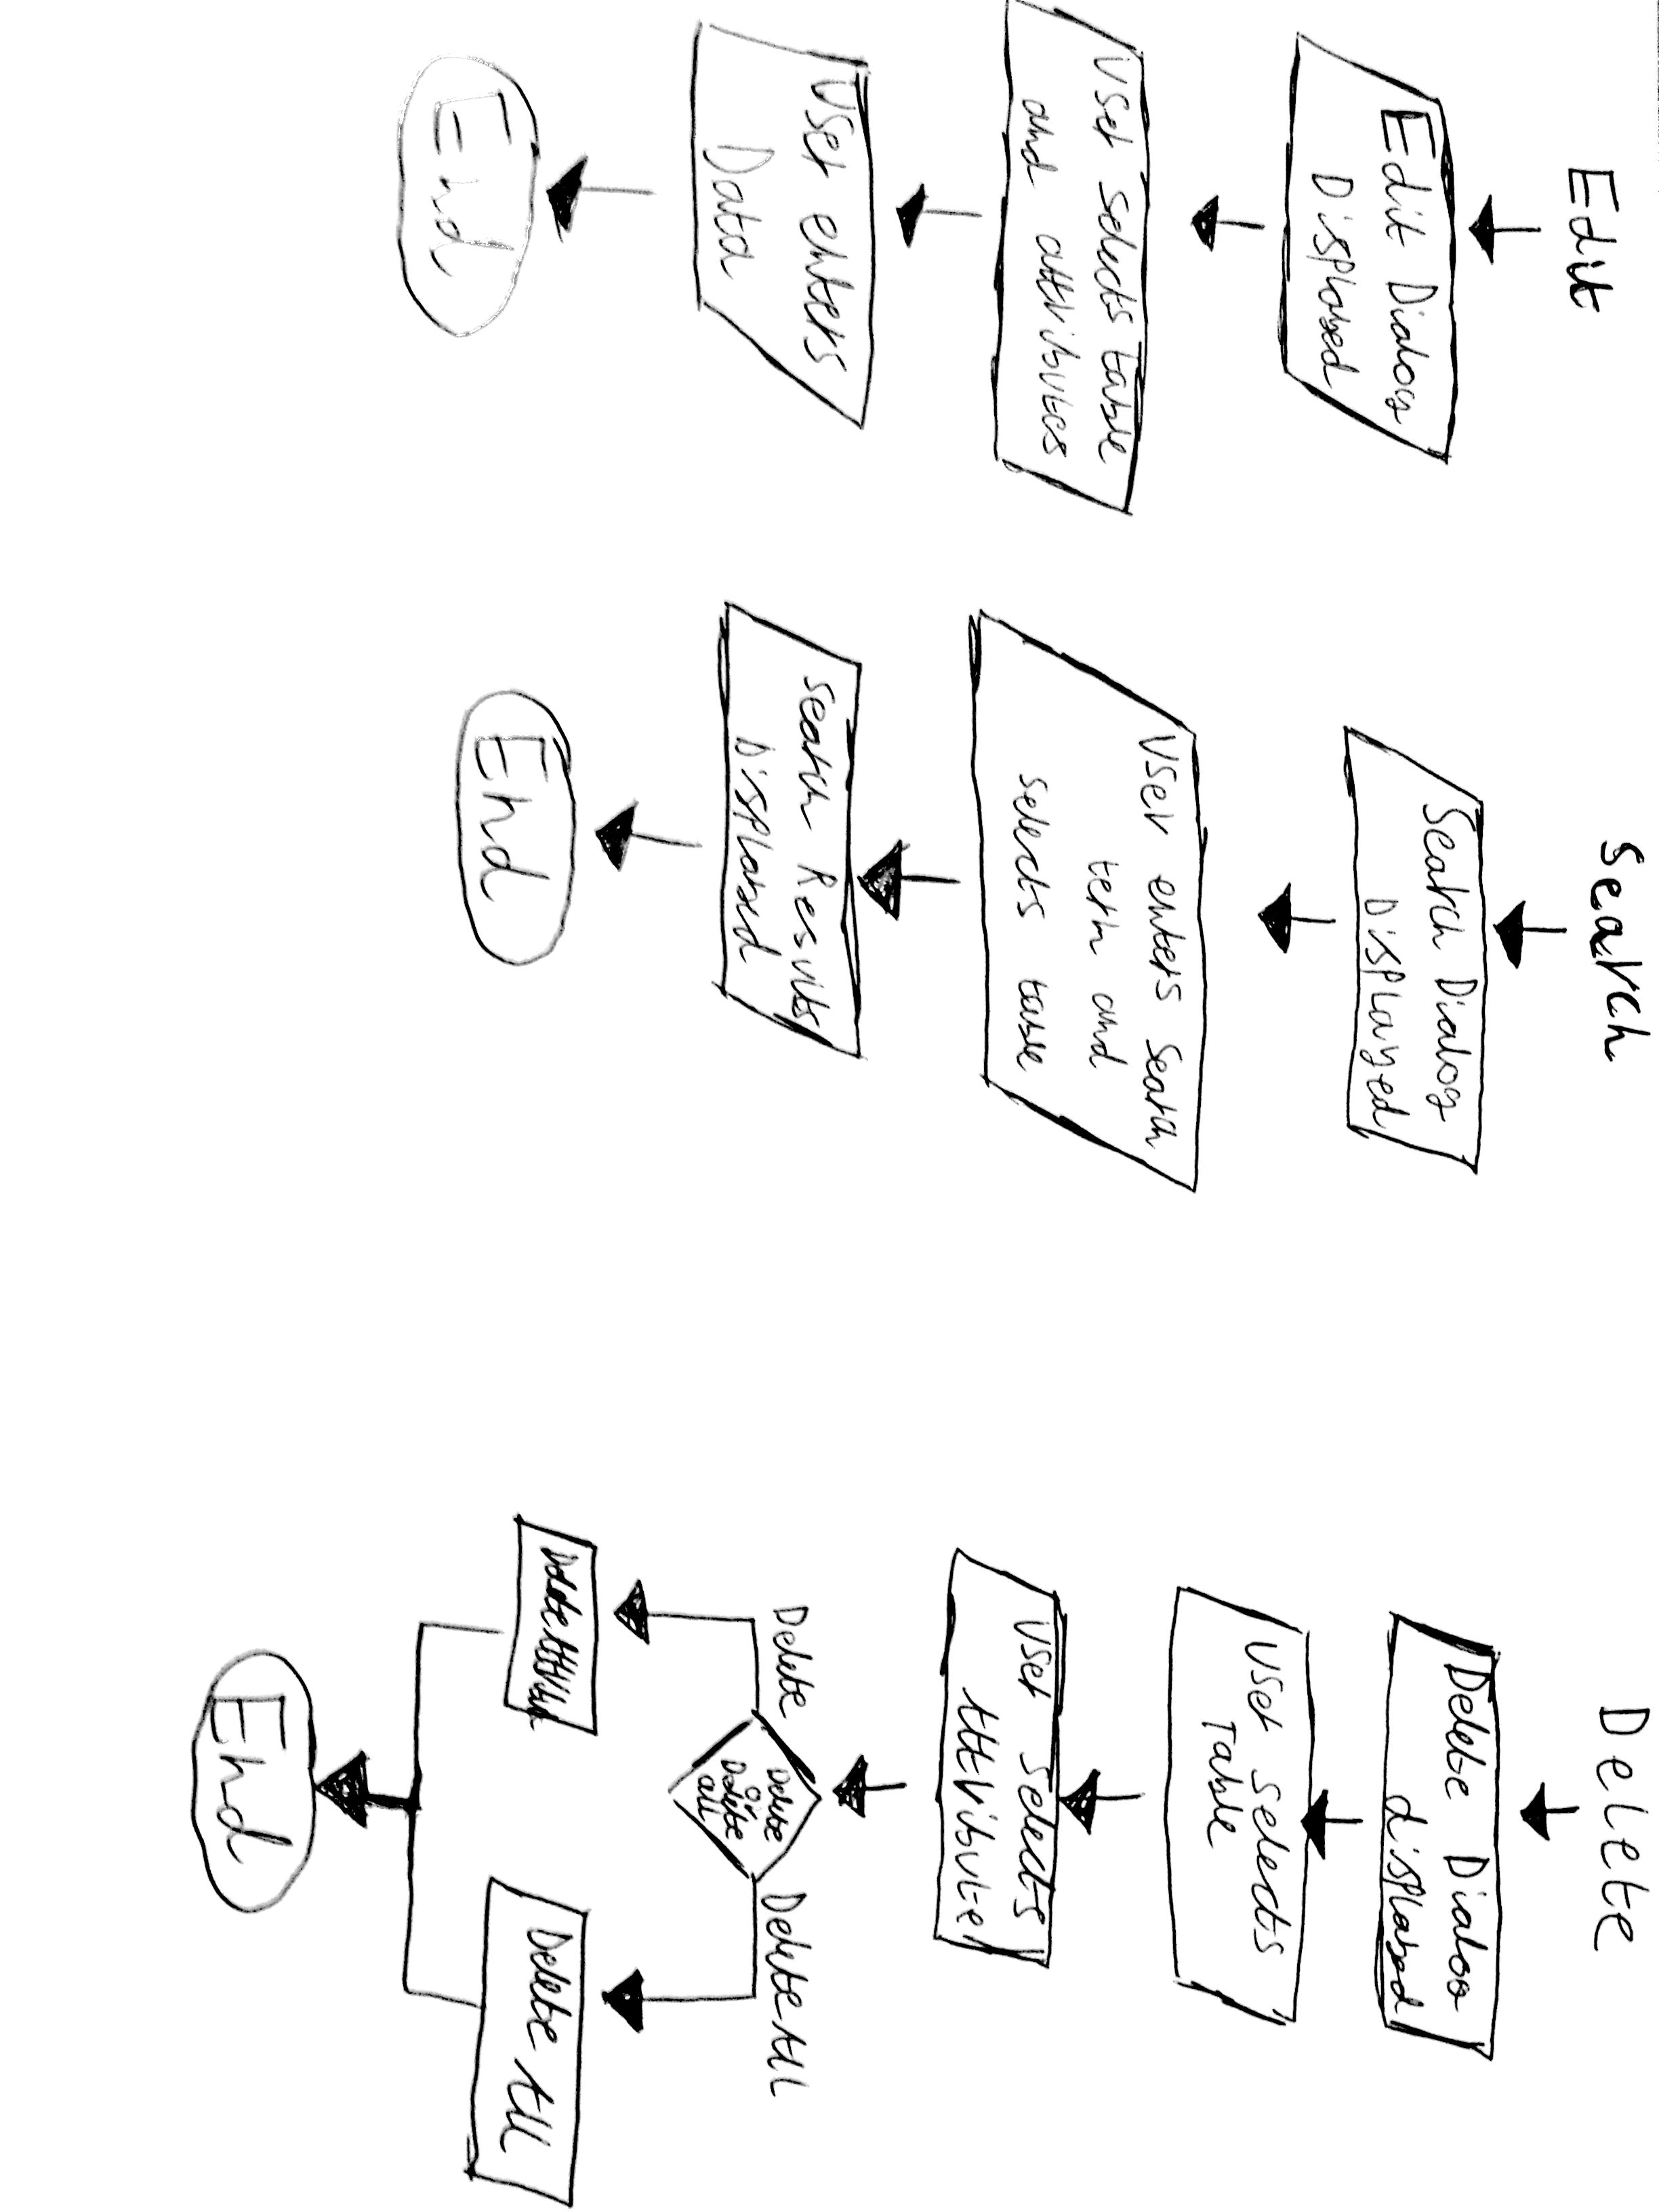
\includegraphics[width=\textwidth]{flowchart 2.jpg}
    \caption{Flowchart} \label{fig:Flowchart}
\end{figure}

\begin{figure}[H]
    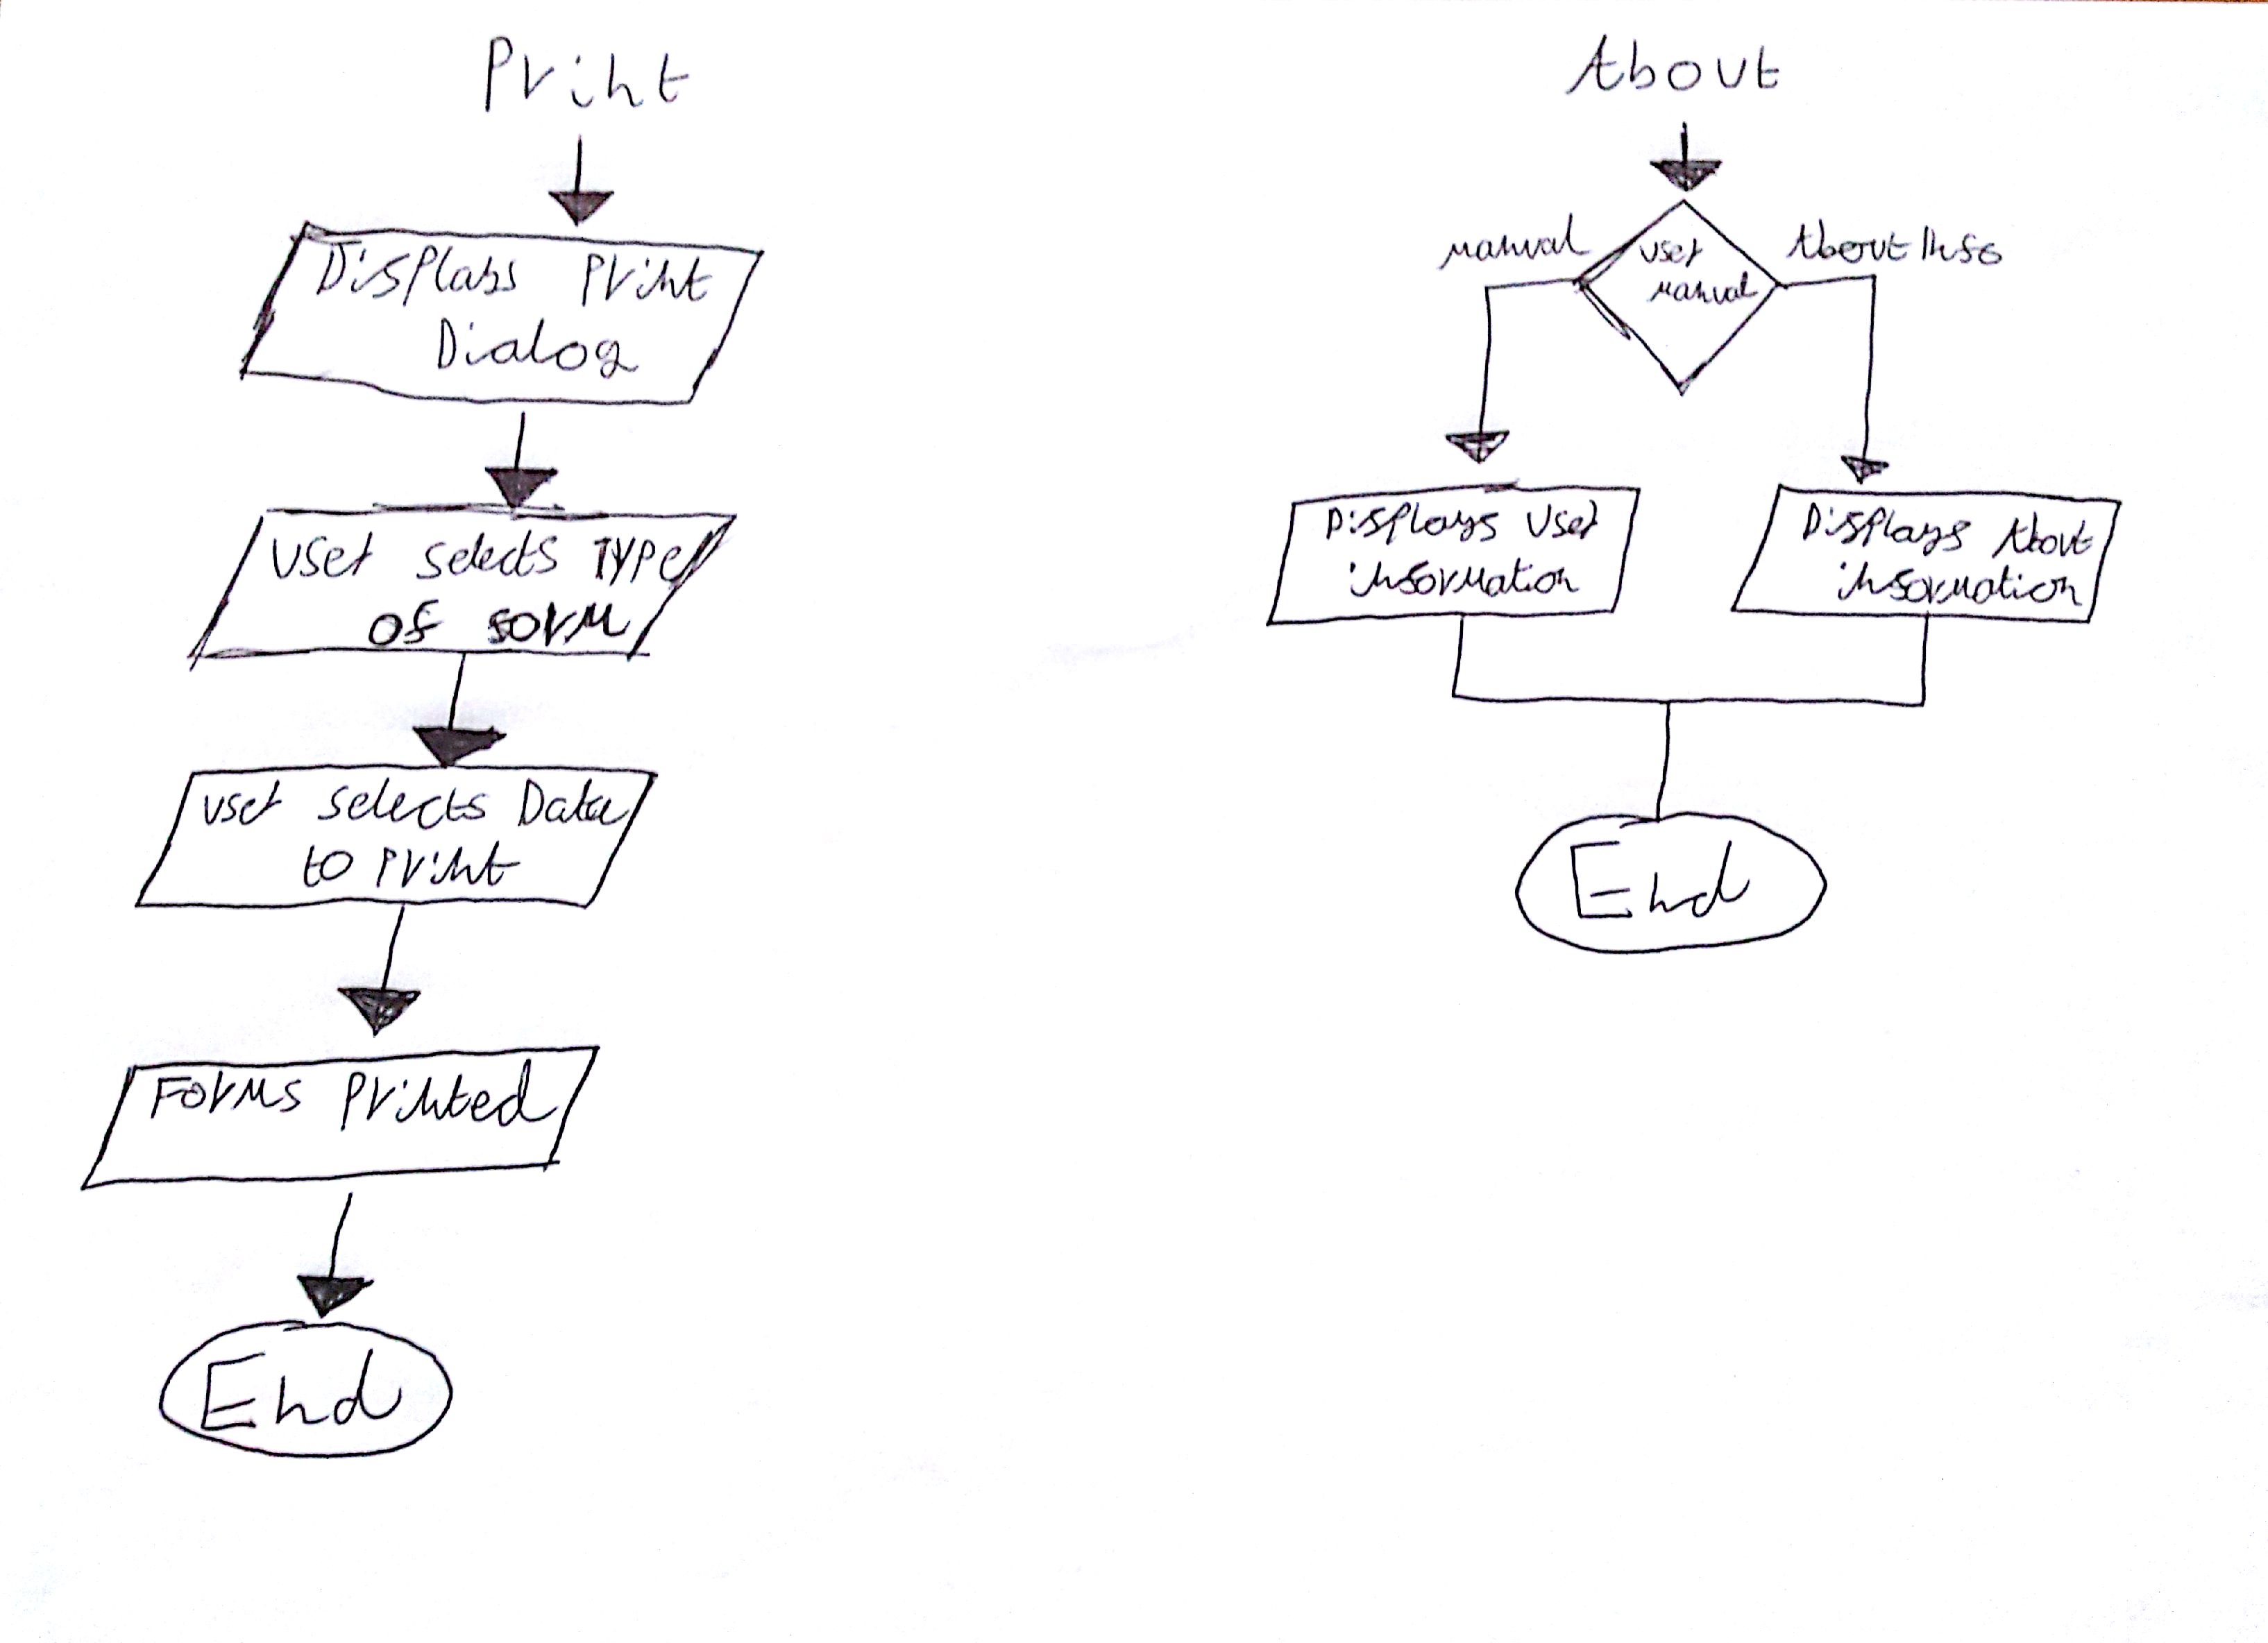
\includegraphics[width=\textwidth]{flowchart1.jpg}
    \caption{Flowchart} \label{fig:Flowchart}
\end{figure}

\section{User Interface Designs}

\begin{figure}[H]
    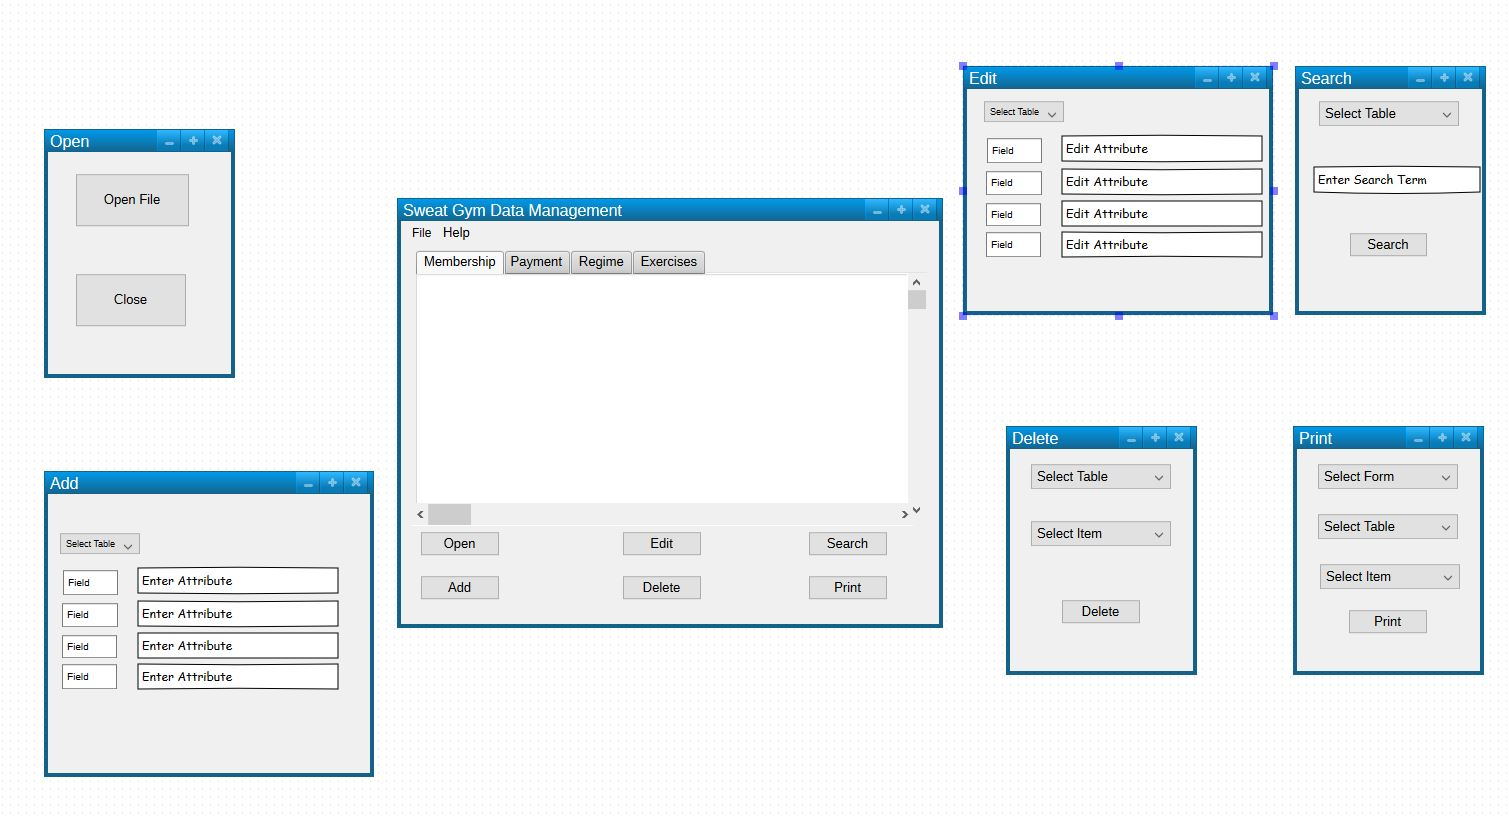
\includegraphics[width=\textwidth]{GUI_DESIGNS.JPG}
    \caption{First Section of GUI} \label{fig:First Section of GUI}
\end{figure}

\begin{figure}[H]
    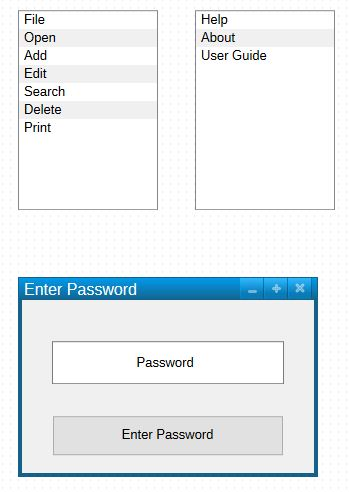
\includegraphics[width=\textwidth]{GUI_DESIGNS_2.jpg}
    \caption{Second Section of GUI} \label{fig:Second Section of GUI}
\end{figure}

\section{Hardware Specification}

The owner currently uses a Notebook laptop powered by an intel 1st generation
i5 processor and 4GB of RAM. He already uses this laptop to run his current
system which uses more resources and power than this system will hopefully
require, but if not he still has more than enough horse power to run the new
system. His use of a laptop is convienient as it means his system is portable
so he doesn’t need to do any data entry (if required) confined to his office and
away from his client if he doesn’t want too and it also means he has a battery so
in the case of a power outtage he wont lose any data. Though it is worth noting
that he may soon be upgrading to a more powerful desktop soon so while this
lowers portability, he has more power for the proposed system and he can easily
have a battery backup in the form of a UPS(Uninterptable Power Supply).
All members will be running this program off the same workstation so the
databases will be stored locally. This wont be a problem as the laptop has a 500 gb hard drive that wont be filled up too quickly and has lots of room for databases and the program. The program will be ouput through a display (like the one used in the laptop) and the program will be operated and have data inputed using mouse/trackpad and keyboard (also contained within my clients laptop). 



\section{Program Structure}

\subsection{Top-down design structure charts}

\begin{figure}[H]
    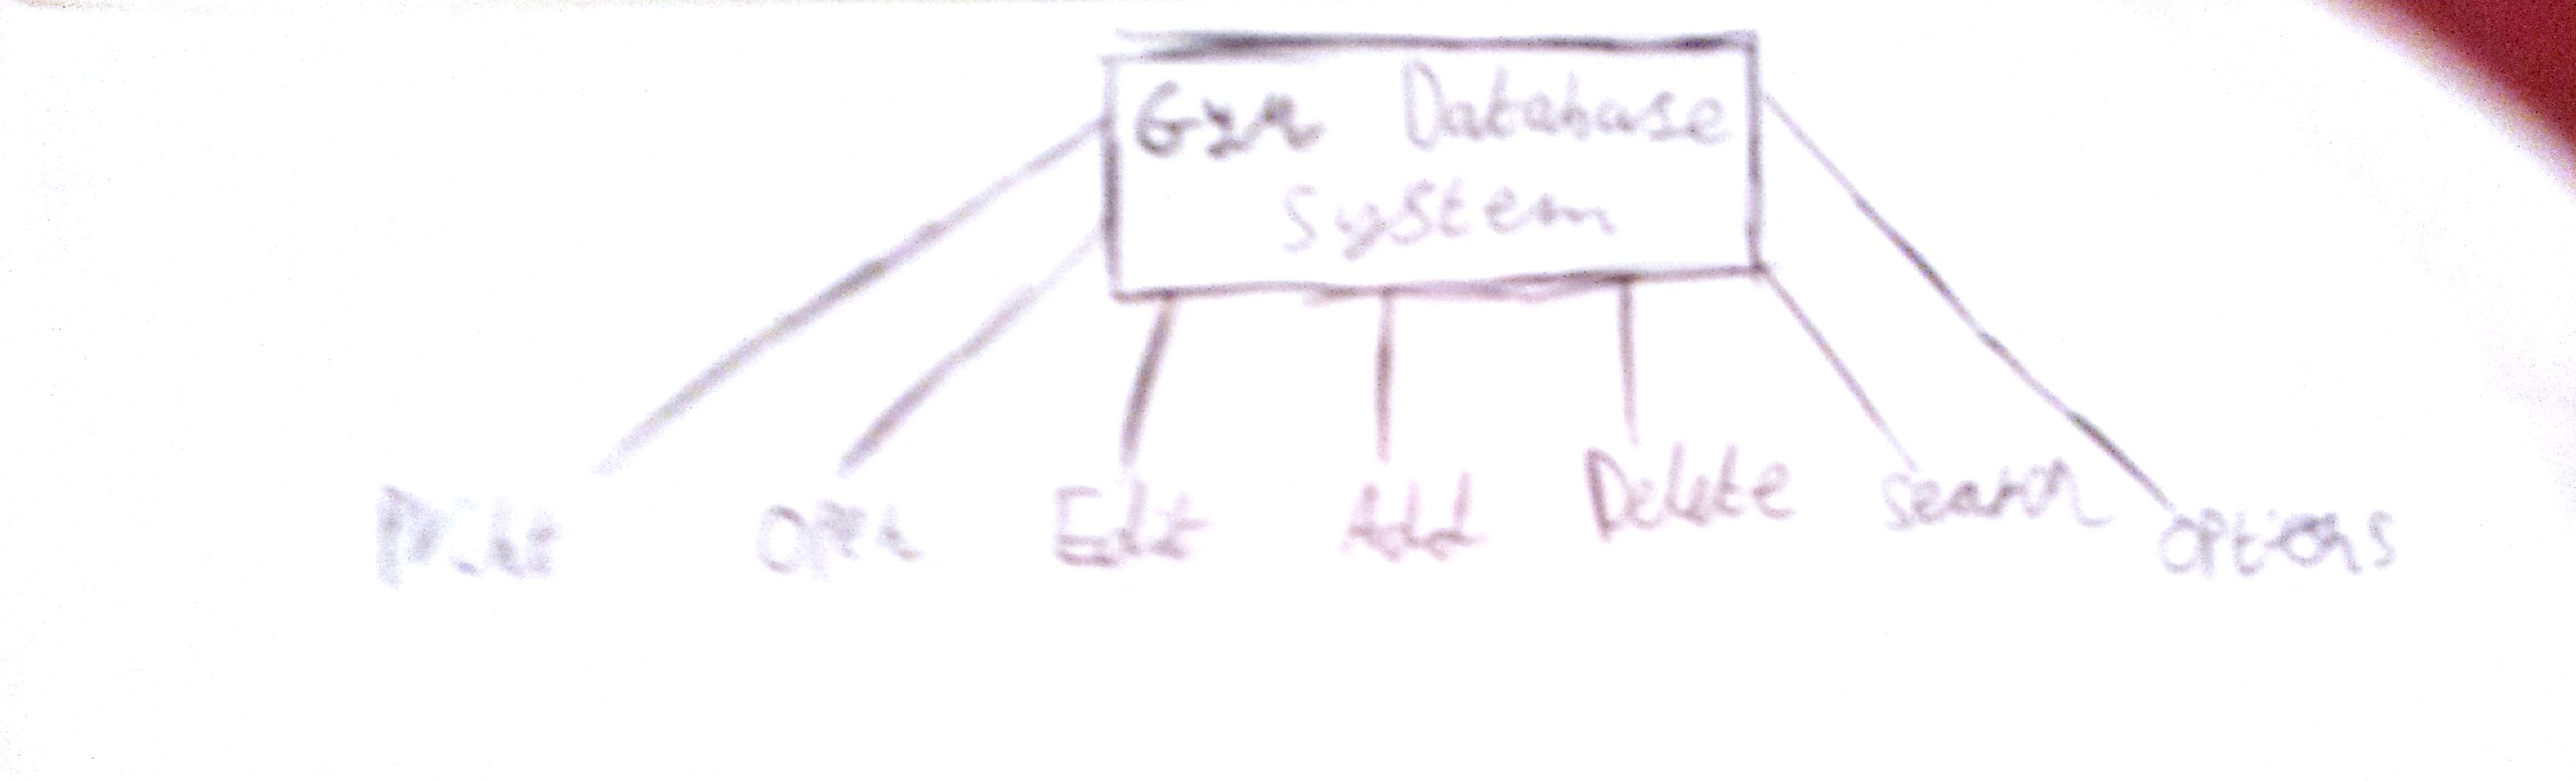
\includegraphics[width=\textwidth]{StructureChart1.jpg}
    \caption{Structure Chart} \label{fig:StructureChart}
\end{figure}

\begin{figure}[H]
    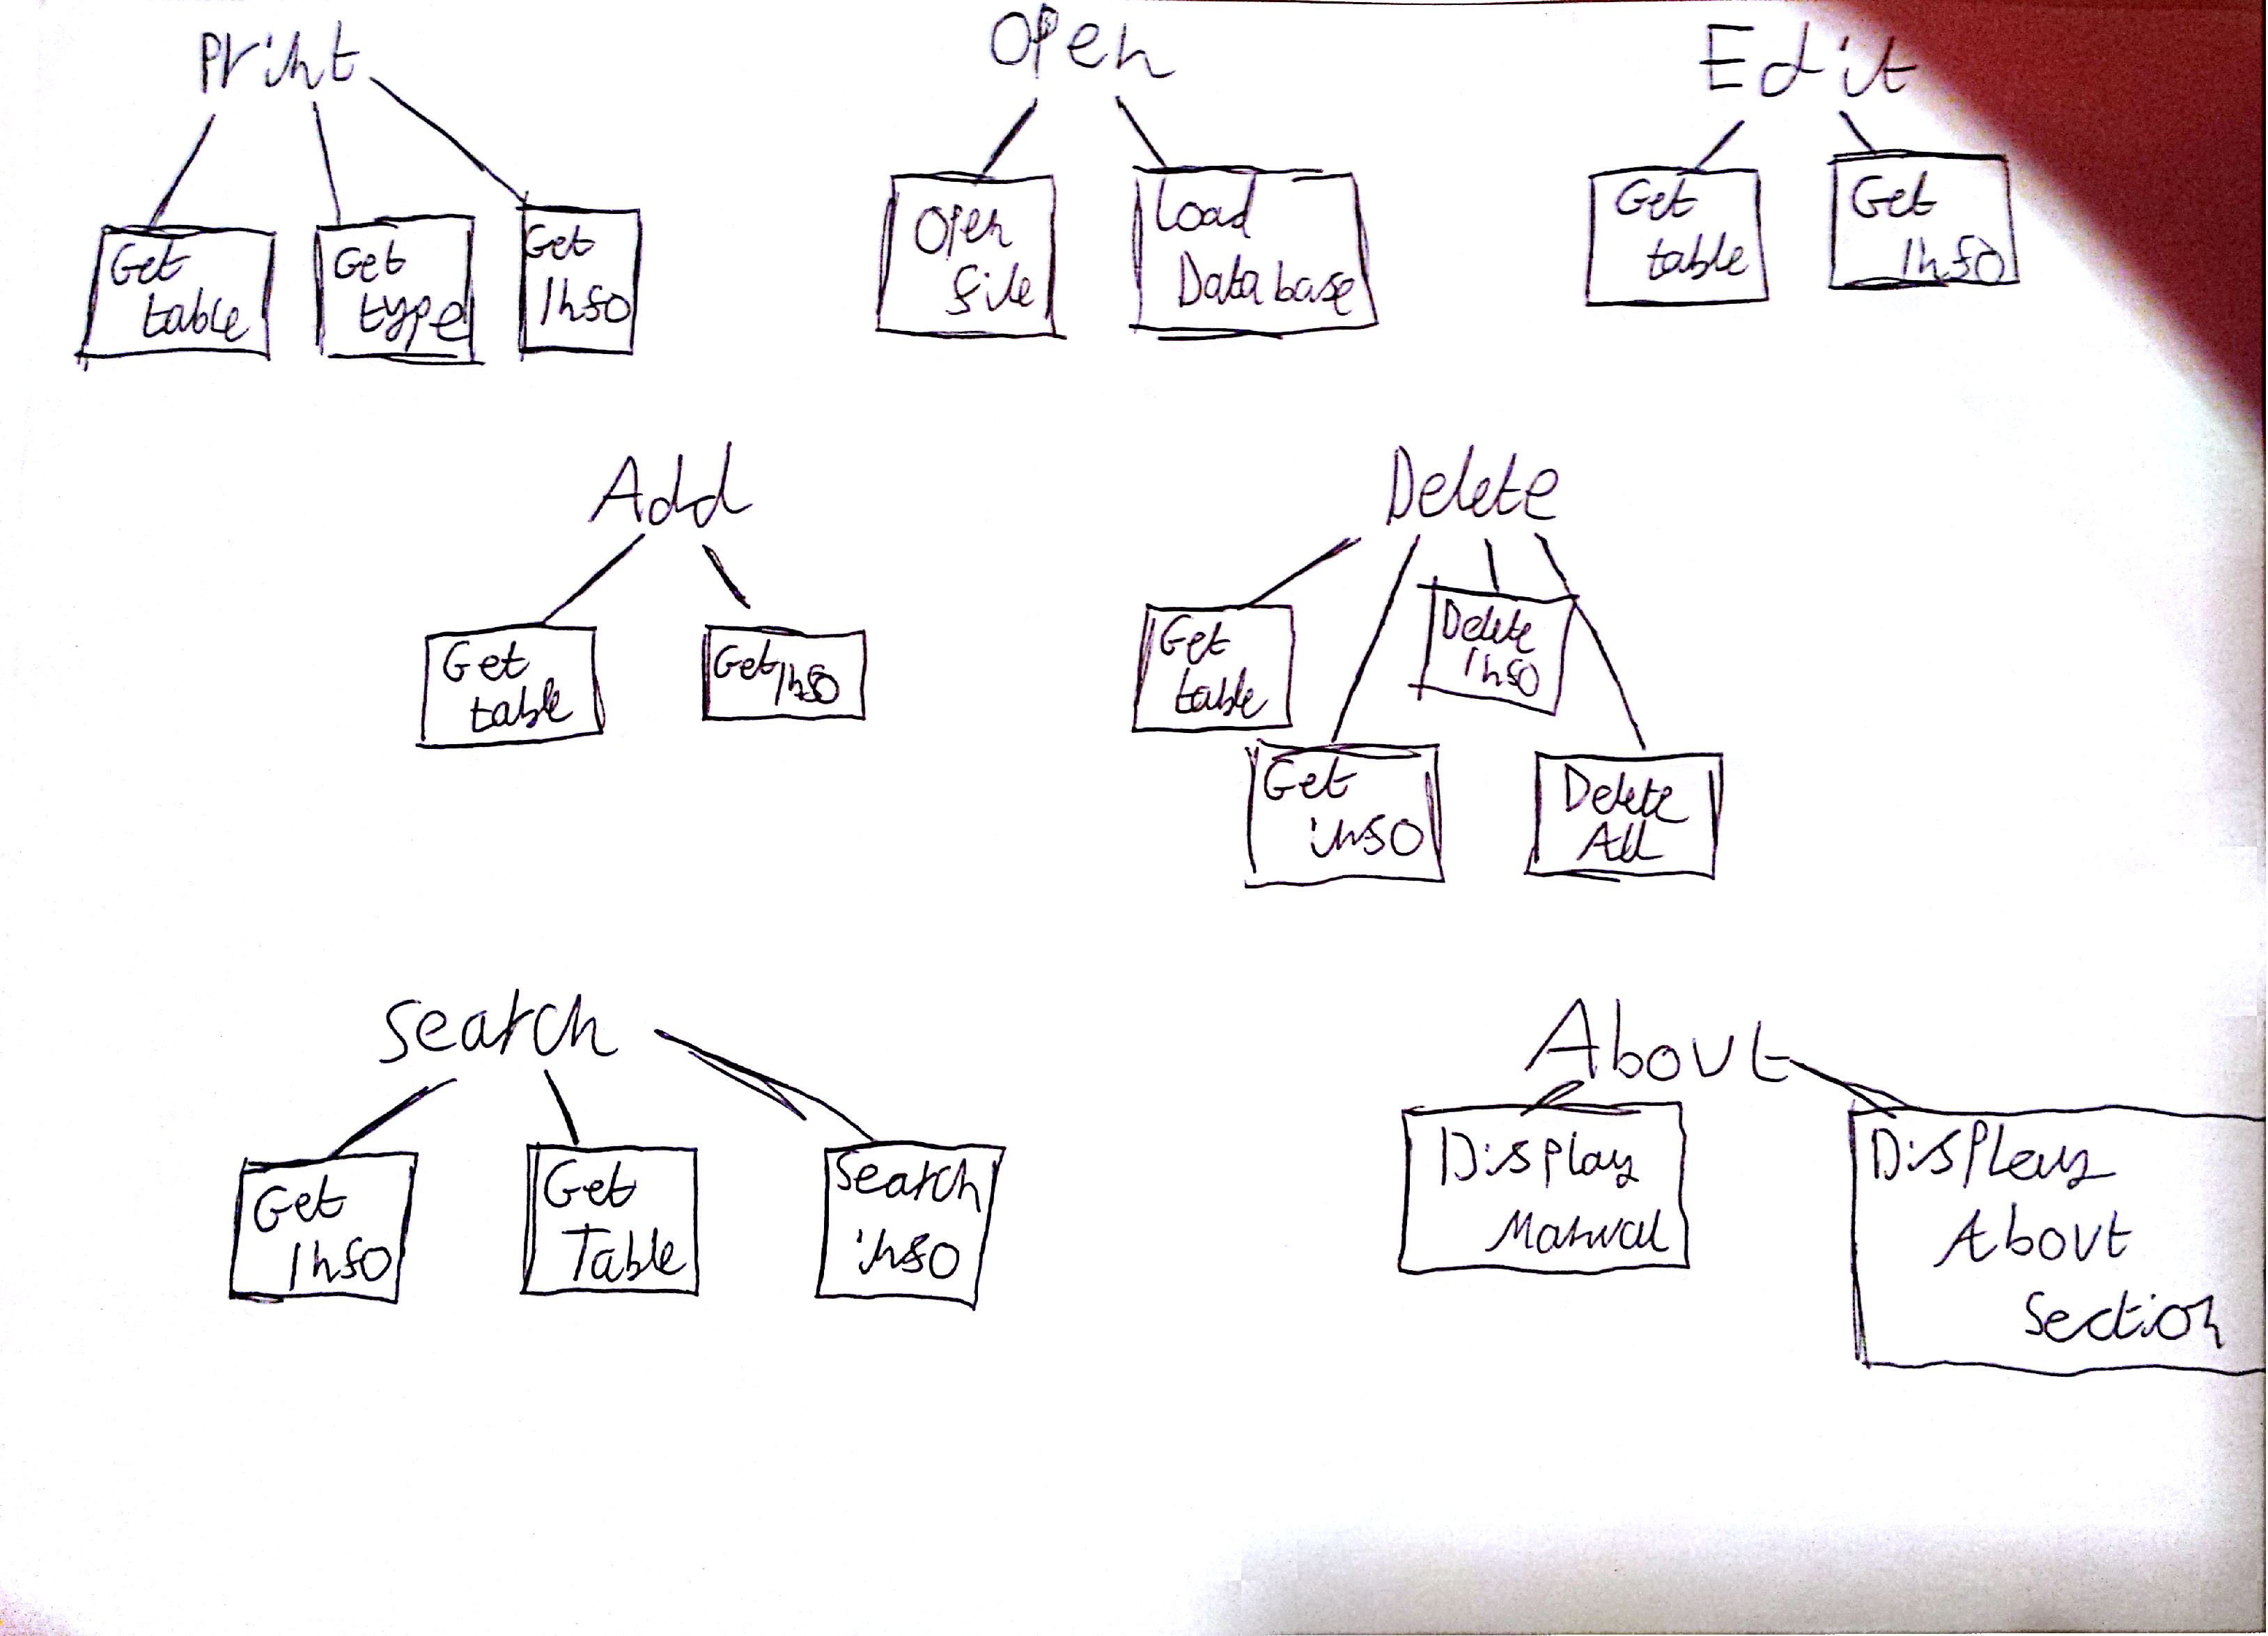
\includegraphics[width=\textwidth]{StructureChart2.jpg}
    \caption{Structure Chart} \label{fig:StructureChart}
\end{figure}



\subsection{Algorithms in pseudo-code for each data transformation process}

\subsection{Object Diagrams}

\subsection{Class Definitions}

\section{Prototyping}

\section{Definition of Data Requirements}

\subsection{Identification of all data input items}

\subsection{Identification of all data output items}

\subsection{Explanation of how data output items are generated}

\subsection{Data Dictionary}

\subsection{Identification of appropriate storage media}

\section{Database Design}

\subsection{Normalisation}

\subsubsection{ER Diagrams}

\subsubsection{Entity Descriptions}

\subsubsection{1NF to 3NF}

\subsection{SQL Queries}

\section{Security and Integrity of the System and Data}

\subsection{Security and Integrity of Data}

\subsection{System Security}

\section{Validation}

\section{Testing}

\begin{landscape}
\subsection{Outline Plan}

\begin{center}
    \begin{tabular}{|p{2cm}|p{5cm}|p{5cm}|p{4cm}|}
        \hline
        \textbf{Test Series} & \textbf{Purpose of Test Series} & \textbf{Testing Strategy} & \textbf{Strategy Rationale}\\ \hline
        Example & Example & Example & Example \\ \hline
    \end{tabular}
\end{center}

\subsection{Detailed Plan}

\begin{center}
    \begin{longtable}{|p{1.5cm}|p{2.5cm}|p{2.5cm}|p{2cm}|p{2cm}|p{2cm}|p{2cm}|p{2cm}|}
        \hline
        \textbf{Test Series} & \textbf{Purpose of Test} & \textbf{Test Description} & \textbf{Test Data} & \textbf{Test Data Type (Normal/ Erroneous/ Boundary)} & \textbf{Expected Result} & \textbf{Actual Result} & \textbf{Evidence}\\ \hline
        Example & Example & Example & Example & Example & Example & Example & Example \\ \hline
    \end{longtable}
\end{center}
\end{landscape}